\lesson{2}{25.09.2023}{Матрицы}
\section{Матрицы}

Пусть v - Это конечно мерно пространство

$v_1 ... v_2$ - базис v

$w \leq V => \exists! v_1, v_2, v_3$

$v = k_1 * v_1 + k_2 * v_2 + k_n * v_n$

\begin{definition}
    $\alpha_1 \alpha_2 \alpha_3$ - координаты

    w в базисе $v_1 v_2$
\end{definition}


$w \leftrightarrow (\alpha_1, \alpha_2 ... \alpha_n)$

$u \leftrightarrow (\beta_1 ... \beta_n)$

$u + w \leftrightarrow (\alpha_1 + \beta_1 * \alpha_2 + \beta_2 ... \alpha_n \beta_n)$

$f * w \leftrightarrow (f * \alpha_1, f * \alpha_2 ... f * \alpha_n)$


$v_1 ... v_n$ - Базис

$u_1, u_2, ... u_n$ - базис

$w = \alpha_1 * v_1 + \alpha_2 * v_2 + \alpha_n * v_n = \beta_1 * u_1 + ... + \beta_n * u_n$

\begin{figure}[H]
    \centering
    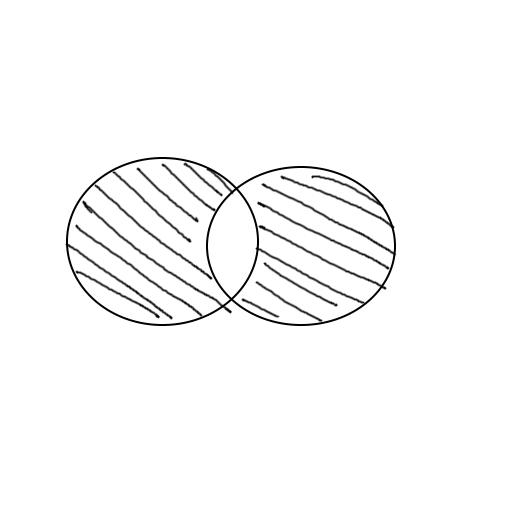
\includegraphics[width=\linewidth]{1.png}
    
    
    \label{fig:1}
\end{figure}

\begin{definition}
    (*)

    $U_1 = a_1 * v_1 + a_2 * v_2 + ... + a_n * v_n$

    $U_2 = a_2 * v_1 + a_2 * v_2 + ... + a_{2n} * v_n$

    \dots

    $U_n = a_n * v_1 + a_{n2} * v_2 + ... + a_{nr} * vn$


\end{definition}



$A = \left(
\begin{array}{ccc}
    a_{11} & \ldots & a_{1m}\\
    \vdots & \ddots & \vdots\\
    a_{n1} &\ldots & a_{nm}
\end{array}
\right)$



матрица перехода от $(v_1 ... v_n) * k $

$u_1 ... u_n$

\begin{definition}
    $A = \left(
    \begin{array}{cccc}
        a_{11} & a_{12} & \ldots & a_{1k}\\
        a_{21} & a_{22} & \ldots & a_{2k}\\
        \vdots & \vdots & \ddots & \vdots\\
        a_{n1} &\ldots & \ldots & a_{nk}
    \end{array}
    \right)$

    Матрица N * R

    $B = \left(
    \begin{array}{cccc}
        b_{11} & b_{12} & \ldots & b_{1l}\\
        b_{21} & b_{22} & \ldots & b_{2l}\\
        \vdots & \vdots & \ddots & \vdots\\
        b_{n1} &\ldots & \ldots & b_{nl}
    \end{array}
    \right)$

    $k \times l$

    $A \cdot B := \left(
        \begin{array}{cccc}
            c_{11} & c_{12} & \ldots & c_{1l}\\
            c_{21} & c_{22} & \ldots & c_{2l}\\
            \vdots & \vdots & \ddots & \vdots\\
            c_{n1} &\ldots & \ldots & c_{nl}
        \end{array}
        \right)$

    $c_{11} = a_{11} * b_{11} + a_{12} * b_{21} + ... + a_{1k} * b_{kl}$

    $c_{12} = a_{11} * b_{12} + a_{12} * b_{22} + ... + a_{1k} * b_{k2}$


\end{definition}

$c_ij := a_{i1} b_{1j} + a_{i2} b_{1y} + ... + a_{zk} b_{kj}$


(*) $\left(
    \begin{array}{c}
        c_{1} \\
        c_{2} \\
        \vdots \\
        c_{n} 
    \end{array}
    \right) \left(
        \begin{array}{ccc}
            a_{11} & \ldots & a_{1n}\\
            \vdots & \ddots & a_{\vdots}\\
            a_{r1} &\ldots & a_{rn}
        \end{array}
        \right) \left(
            \begin{array}{c}
                r_{1}\\
                r_{2}\\
                \vdots\\
                r_{n}
            \end{array}
            \right)$

$w_1 ... w_n$ - базис

$V_! = b_{11} * w_1 + ... + b_{1n} * w_n$

$\dots$

$v_n = b_{n1} * w_1 + \dots b_{nn} * w_n$



$u_q = a_{11} * v_1 + a_{12} v_2 + ... + a_{1n} v_n = a_{11} (b_{11} w_1 + ... + b_{1n} w_n) + ... + a_1n (b_{n1} w_1 + ... + b_{nn} w_n) = w_1 (a_{11} b_{11} + a_{12} b_{21} + ... + a_{1n} b_{n1}) . \dots$

\begin{theorem}
    Если A - Это матрица перехода от $\{v_i\} к \{u_i\}$

    B - матрица перехода от $\{w_i\} к \{v_i\}$

    => $A \cdot B$ - м. п. от $\{w_2\} к \{u_i\}$
\end{theorem}

$A \setminus B: A \cdot B \neq B \cdot A !$

\begin{theorem}
    
    A(BC) = (AB)C 


    Умножение матриц хоть и не коммутативно, но ассоциативно.

\end{theorem}

% волнистая стрелка с C, B, A
$w_1 ... w_n \to v_1 ... v_k \to u_1 ... u_e \to t_1 ... t_m$


$w_1 ... w_n \to w_1 ... w_n$

$\left(
        \begin{array}{ccc}
            1 & \ldots & 0\\
            \vdots & \ddots \vdots\\
            0 & \ldots & 1
        \end{array}
        \right)$ - единичная матрица

$u_1 ... u_n$ - базис

$v_1 ... v_n$ - базис

$\left(
        \begin{array}{c}
            u_1\\
            \vdots\\
            u_n
        \end{array}
        \right) = A \left(
            \begin{array}{c}
                r_1\\
                \vdots\\
                r_n
            \end{array}
            \right)$


$\left(
    \begin{array}{c}
        r_1\\
        \vdots\\
        r_n
    \end{array}
    \right) = B \left(
        \begin{array}{c}
            u_1\\
            \vdots\\
            u_n
        \end{array}
        \right)$

$A \cdot B = E$

$B \cdot A = E$

(A и B) - обратные матрицы

\section{Скалярное произведение}

\begin{definition}
    V - векторное пространство

    ($\cdot, \cdot$) : $V \times V \to \R$

    \begin{enumerate}
        \item (u, u) $\geq 0$
        (u, u) = 0 <=> U = 0

        \item $(u_1 + u_2; v) = (u_1, v_1) + (u_2, v)$
        $(u, v_1 + v_2) = (u_, v_1) + (u_1 v_2)$

        \item $\alpha(u, v) = (\alpha u, v) = (u, \alpha v)$
        \item (u, v) = (v, u)
    \end{enumerate}

    V - евклидово пространство
    $(\cdot, \cdot)$ - скалярное произведение
\end{definition}

Для комплексных чисел 4L

$(u, v) = \overline{(v, u)}$

$(u, \alpha v) = \overline{\alpha} (u, v)$

\begin{eg}
    \begin{enumerate}
        \item $ V = \R^n $
        
        $(a_1, a_2, ..., a_n) + (b_1, b_2, ..., b_n) := a_1 b_1 + a_2 b_2 + ... + a_n b_n$

        
    $\left(
    \begin{array}{ccc}
        a_1 & \ldots & a_n
    \end{array}\right) \left(
                \begin{array}{c}
                    a_1\\
                    \vdots\\
                    a_n
                \end{array}
                \right)$

        \item V - пространство функций (...) 
        $(f(x), g(x)) := \int_a^b f(x)g(x)dx$
    \end{enumerate}
\end{eg}

\begin{definition}
    Пускай V - евклидово пространство

    v - элемент V

    $|v| := \sqrt{ (v, v) }$

    $cos @a(u, v) := \frac{(u, w)}{|u| \cdot |v|}$

    (u, v + 0)


\end{definition}

\begin{theorem}(Неравенство КБШ)

    $|(u, w)| \leq |u| \cdot |v|$

\end{theorem}

$0 \leq (\overline u + f \overline v; \overline u + f \overline v) = (\overline u, \overline u) + (\overline u, t \overline v) + (t \overline v, \overline u)+ \forall t + (t \overline v, t \overline u) = t^2 (v, v) + 2t(u;v) + (u, u)$

$D \leq 0$

$\frac{D}{u} = (u; v)^2 - (u. u)(v, v) \leq 0$

$(u, v)^2 \leq (u, u) \cdot v, v$

\begin{definition}
    \begin{enumerate}
        \item $|a_1 b_1 + a_2 b_2 + ... + a_n b_n| \leq \sqrt{a_1^2 + a_2^2 + ... + a_n^2} \sqrt{b_1^2 + b_2^2 + ... + b_n^2}$
        
        \item $(\int_a^b f(x)g(x)dx)^2 \leq (\int_a^b g(x)dx)$
    \end{enumerate}
\end{definition}


 \begin{definition}
    $u \perp v$, если $(u, b) = 0$
 \end{definition}

 $v_1 ... v_n$ - ортогональная, если 

 $v_i \perp v_j (i \neq j)$

 \begin{theorem}
    $v_1 ... v_n$ - ортогональная система, нет нулевых векторов

    => $v_1 ... v_n$ линейно не зависимы.
 \end{theorem}

 \begin{proof}
    
    $\alpha_1 v_1 + ... + \alpha_n v_n = 0$

    $(v_1 v_i) = 0$
    $\alpha_1 (v_1 v_i) + \alpha_2 (v_2, v_i) + ... + \alpha_i (v_1, v_i) + ... = 0$
    
    $a_i (v_i)^2 = 0$

    $\alpha_i = 0$
 \end{proof}

 \begin{definition}
    u - нормированый или единичный если $|u| = 1$

    $v_1 ... v_n$ - ортонормированные системы, если $v_i \perp v_j$ и $|v_i| = 1$

    $v_1 .. v_i$ - ОНБ ортонормированный базис
 \end{definition}